\documentclass[times,specification,annotation]{itmo-student-thesis}

\usepackage{icomma}
\usepackage[T2A]{fontenc}
\usepackage[utf8]{inputenc}
\usepackage[russian]{babel}

\usepackage{tikz}
\usetikzlibrary{arrows}
\usepackage{filecontents}
\usepackage{listings}
\usepackage{wrapfig}
\usepackage{biblatex}
\begin{filecontents}{reference.bib}
@inproceedings{ku04,
    author = {Ku, KM and Ha, KJ and Yoo, WH and Koo, KY},
    year = {2004},
    month = {01},
    pages = {196-205},
    title = {Parallel Montgomery multiplication and squaring over GF(2(m)) based on cellular automata},
        langid      = {english},
    isbn = {3-540-22060-7}
}

@inproceedings{mau15,
    author = {Maulana, Mirza and Senjaya, Wenny and Rahardjo, Budi and Muchtadi-Alamsyah, Intan and Paryasto, Marisa},
    year = {2015},
    month = {01},
    pages = {},
    title = {Implementation of Finite Field Arithmetic Operations for Polynomial and Normal Basis Representations},
    doi = {10.2991/iccst-15.2015.25},
    langid = {english}
}

@article{koc97,
    author = {Koc, Cetin and Acar, T.},
    year = {1997},
    month = {01},
    pages = {225},
    title = {Fast Software Exponentiation in GF(2^k)},
    volume = {0},
    isbn = {0-8186-7846-1},
    journal = {Computer Arithmetic, IEEE Symposium on},
        langid      = {english},
    doi = {10.1109/ARITH.1997.614899}
}

@article{koc98,
    author = {Koc, Cetin and Acar, Tolga},
    year = {1998},
    month = {04},
    pages = {57-69},
    title = {Montgomery Multiplication in GF(2k)},
    volume = {14},
    journal = {Designs Codes and Cryptography},
    langid      = {english},
    doi = {10.1023/A:1008208521515}
}

@article{adr15,
    author = {Adrian, David and Bhargavan, Karthikeyan and Durumeric, Zakir and Gaudry, Pierrick and Green, Matthew and Halderman, J. and Heninger, Nadia and Springall, Drew and Thomé, Emmanuel and Valenta, Luke and Vandersloot, Benjamin and Wustrow, Eric and Zanella-Béguelin, Santiago and Zimmermann, Paul},
    year = {2015},
    month = {10},
    pages = {},
    title = {Imperfect Forward Secrecy: How Diffie-Hellman Fails in Practice},
    volume = {62},
    journal = {Communications of the ACM},
    langid = {english},
    doi = {10.1145/3292035}
}

@article{dif77,
  abstract = {Two kinds of contemporary developments in cryptography are examined. Widening applications of teleprocessing have given rise to a need for new types of cryptographic systems, which minimize the need for secure key distribution channels and supply the equivalent of a written signature. This paper suggests ways to solve these currently open problems. It also discusses how the theories of communication and computation are beginning to provide the tools to solve cryptographic problems of long standing.},
  added-at = {2009-01-14T00:43:43.000+0100},
  author = {Diffie, Whitfield and Hellman, Martin E.},
  journal = {IEEE Transactions on Information Theory},
  keywords = {imported},
  month = {November},
  number = 6,
  pages = {644-654},
  timestamp = {2009-01-14T00:43:46.000+0100},
  title = {New Directions in Cryptography},
  topic = {diffiehellman[1]},
  uri = {http://www.cs.purdue.edu/homes/ninghui/courses/Fall04/lectures/diffie-hellman.pdf},
  volume = 22,
    langid      = {english},
  year = 1976
}

@article{zhu17,
    author = {Алексей Евгеньевич Жуков},
    journal = {Вопросы кибербезопасности},
    number = {3 (21)},
    pages = {70-76},
    title = {Клеточные автоматы в криптографии. Часть 1},
    uri = {https://cyberleninka.ru/article/n/kletochnye-avtomaty-v-kriptografii-chast-1},
    langid = {russian},
    doi = {10.21581/2311-3456-2017-3-70-76},
    year = 2017
}

@article{zhu17_2,
    author = {Алексей Евгеньевич Жуков},
    journal = {Вопросы кибербезопасности},
    number = {4 (22)},
    pages = {47-66},
    title = {Клеточные автоматы в криптографии. Часть 2},
    uri = {https://cyberleninka.ru/article/n/kletochnye-avtomaty-v-kriptografii-chast-2},
    langid = {russian},
    doi = {10.21581/2311-3456-2017-4-47-66},
    year = 2017
}

@article{pri16,
  title={Разработка алгебраической библиотеки конечных полей для обобщенных криптографических алгоритмов},
  author={Приньков, АС and Николаев, ДА},
  journal={Международный научно-исследовательский журнал},
  number={7 (49) Часть 4},
  pages={92--94},
  langid = {russian},
  year={2016}
}

@article{jeo07,
    author = {Jeon, Jun-Cheol and Kee-Young, Yoo},
    year = {2007},
    month = {03},
    pages = {915-922},
    title = {Programmable cellular automata based Montgomery hardware architecture},
    volume = {186},
    journal = {Applied Mathematics and Computation},
    langid = {english},
    doi = {10.1016/j.amc.2006.08.018}
}

@book{knu97,
    author = {Knuth, Donald E.},
    title = {The Art of Computer Programming, Volume 1 (3rd Ed.): Fundamental Algorithms},
    year = {1997},
    isbn = {0201896834},
    publisher = {Addison Wesley Longman Publishing Co., Inc.},
    langid      = {english},
    address = {USA}
}

@book{knu97_2,
  added-at = {2015-06-04T07:16:19.000+0200},
  address = {Boston},
  author = {Knuth, Donald E.},
  biburl = {https://www.bibsonomy.org/bibtex/25dbc415549a1bb86bff7a3842765c31f/ytyoun},
  interhash = {b825ccd550f92a93eefbacd1bec78704},
  intrahash = {5dbc415549a1bb86bff7a3842765c31f},
  isbn = {0201896842 9780201896848},
  keywords = {algorithm knuth no.pdf taocp textbook},
  publisher = {Addison-Wesley},
  refid = {174763889},
    langid      = {english},
  timestamp = {2015-07-29T09:31:05.000+0200},
  title = {The Art of Computer Programming, Volume 2 (3rd Ed.): Seminumerical Algorithms},
  year = 1997
}

@book{men01,
  added-at = {2007-04-16T14:16:26.000+0200},
  author = {Menezes, Alfred J. and van Oorschot, Paul C. and Vanstone, Scott A.},
  biburl = {https://www.bibsonomy.org/bibtex/21fb86a3afb62bbb4bc2f94a0299a4d59/kidloc},
  interhash = {d5837a554ce2ffd49f551045400e244c},
  intrahash = {1fb86a3afb62bbb4bc2f94a0299a4d59},
  keywords = {cryptography handbook programming reference security},
  publisher = {CRC Press},
  timestamp = {2007-04-16T14:16:26.000+0200},
  title = {Handbook of Applied Cryptography},
  url = {http://www.cacr.math.uwaterloo.ca/hac/},
  langid = {english},
  year = 2001
}

@book{sma15,
    author = {Smart, Nigel P.},
    title = {Cryptography Made Simple},
    year = {2015},
    isbn = {3319219359},
    publisher = {Springer Publishing Company, Incorporated},
    edition = {1st},
    doi = {10.5555/2927491},
    langid = {english},
}

@misc{rfc2412,
	series =	{Request for Comments},
	number =	2412,
	howpublished =	{RFC 2412},
	publisher =	{RFC Editor},
	doi =		{10.17487/RFC2412},
	url =		{https://rfc-editor.org/rfc/rfc2412.txt},
    author =	{Hilarie Orman},
	title =		{{The OAKLEY Key Determination Protocol}},
	pagetotal =	55,
	year =		1998,
	month =		nov,
    langid      = {english},
}

@misc{rfc7296,
	series =	{Request for Comments},
	number =	7296,
	howpublished =	{RFC 7296},
	publisher =	{RFC Editor},
	doi =		{10.17487/RFC7296},
	url =		{https://rfc-editor.org/rfc/rfc7296.txt},
    author =	{Charlie Kaufman and Paul E. Hoffman and Yoav Nir and Pasi Eronen and Tero Kivinen},
	title =		{{Internet Key Exchange Protocol Version 2 (IKEv2)}},
	pagetotal =	142,
	year =		2014,
	month =		oct,
    langid      = {english},
}

@misc{rfc3526,
	series =	{Request for Comments},
	number =	3526,
	howpublished =	{RFC 3526},
	publisher =	{RFC Editor},
	doi =		{10.17487/RFC3526},
	url =		{https://rfc-editor.org/rfc/rfc3526.txt},
    author =	{Mika Kojo and Tero Kivinen},
	title =		{{More Modular Exponential (MODP) Diffie-Hellman groups for Internet Key Exchange (IKE)}},
	pagetotal =	10,
	year =		2003,
	month =		may,
    langid      = {english},
}

\end{filecontents}
%% Конец

%% Указываем файл с библиографией.
\addbibresource{reference.bib}

\begin{document}

\studygroup{N3451}
\faculty{ФБИТ}
\specialty{10.03.01 Информационная безопасность}
\specialization{Организация и технология защиты информации}
\title{Разработка модификации алгоритма Диффи-Хеллмана c
    использованием клеточных автоматов}
\author{Крикун Александр Артемович}{Крикун А.А.}
\supervisor{Левина Алла Борисовна}{Левина А.Б.}{к.физ-мат.н.}{доцент, Университет ИТМО}
\publishyear{2020}
%% Дата выдачи задания. Можно не указывать, тогда надо будет заполнить от руки.
\startdate{23}{ноября}{2019}
%% Срок сдачи студентом работы. Можно не указывать, тогда надо будет заполнить от руки.
\finishdate{31}{мая}{2020}
%% Дата защиты. Можно не указывать, тогда надо будет заполнить от руки.
%% \defencedate{15}{июня}{2019}
\secretary{Коваль Е.Н.}

%% Задание
%%% Техническое задание и исходные данные к работе
\technicalspec{
Цель работы – оптимизация алгоритма Диффи-Хеллмана с помощью распараллеливания алгоритма возведения в степень Монтгомери для применения с ключами большего размера.
Для достижения цели необходимо:
\begin{enumerate}[label=\arabic*.]
    \item Провести анализ алгоритма Диффи-Хеллмана.
    \item Провести анализ известных методов оптимизации шагов алгоритма с помощью клеточных автоматов.
    \item Разработать программную реализацию модификации алгоритма возведения в степень Монтгомери, оптимизированного с помощью параллельных вычислений.
    \item Разработать программную реализацию алгоритма с использованием оптимизированных элементов.
    \item Провести оценку полученных результатов.
\end{enumerate}
}

%%% Содержание выпускной квалификационной работы (перечень подлежащих разработке вопросов)
\plannedcontents{
\begin{enumerate}[label=\arabic*.]
    \item Анализ алгоритма Диффи-Хеллмана и задачи быстрого возведения в степень.
    \item Детальный анализ распараллеливания алгоритма возведения в степень Монтгомери.
    \item Программная реализация оптимизированного алгоритма.
    \item Оценка полученных результатов.
\end{enumerate}
}

\plannedgraphics{
\begin{enumerate}[label=\arabic*.]
    \item Схема алгоритма Диффи-Хеллмана.
    \item Схема алгоритма побитового возведения в степень Монтгомери.
    \item Схема параллелизованного алгоритма побитового возведения в степень Монтгомери.
\end{enumerate}
}

%%% Исходные материалы и пособия
\plannedsources{
\begin{enumerate}[label=\arabic*.]
    \item Paar C. Understanding Cryptography. C. Paar – М.: Springer; 2014. – 392с.
    \item \c{C}.K. Ko\c{c}, T. Acar, Montgomery Multiplication in GF$\left(2^k\right)$,
    Kluwer Academic Publishers, Designs, Codes and Cryptography, 14(1), pp. 57-69, April 1998..
    \item \c{C}.K. Ko\c{c}, T. Acar, Fast software exponentiation in GF$\left(2^k\right)$
    In \emph{Proceedings, 9th Symposium on Computer Arithmetic}, pages 225–231, Asilomar, California, July 6–9, 1997
    \item Menezes A, Oorschot PV, Vanstone S.
    (1997) Handbook of applied cryptography.
    CRC, Boca Raton.
    \item K. Ku, K. Ha, W. Yoo, and K. Yoo, ``Parallel Montgomery multiplication and squaring over GF$\left(2^m\right)$ Based on cellular automata'',
    Proc. ICCSA 2004, (LNCS, 3046), pp. 196-205, 2004
\end{enumerate}
}

%%% Цель исследования
\researchaim{Оптимизация алгоритма Диффи-Хеллмана с использованием параллельного алгоритма
    возведения в степень Монтгомери для применения на пространстве ключей до 4 килобит.}

%%% Задачи, решаемые в ВКР
\researchtargets{\begin{enumerate}
    \item Анализ алгоритма Диффи-Хеллмана.
    \item Анализ известных методов оптимизации шагов алгоритма с помощью клеточных автоматов.
    \item Разработка программной реализации модификации алгоритма возведения в степень Монтгомери, оптимизированного с помощью параллелизма.
    \item Разработка программной реализации алгоритма с использованием оптимизированного возведения в степень.
    \item Тестирование производительности и оценка полученных результатов.
\end{enumerate}}

%%% Использование современных пакетов компьютерных программ и технологий
\addadvancedsoftware{Python 3.7}{\ref{sec:prog}-\ref{sec:results}, Приложение~\ref{sec:app:1}}
\addadvancedsoftware{Matplotlib 3.1.3}{\ref{sec:results}}

%%% Краткая характеристика полученных результатов
\researchsummary{В рамках дипломной работы была реализована открытая библиотека для вычислений в конечных полях,
которая включала как традиционные, так и оптимизированные \\алгоритмы возведения в степень по модулю.
Были реализованы модификации алгоритма Диффи-Хеллмана, использующие алгоритмы слева-направо, Монтгомери и параллельный Монтгомери.
Также были проведены тесты на \\сравнение производительности модификаций.
Предложенная в работе оптимизация позволяет получить прирост производительности как минимум в 40 по сравнению со стандартной версией алгоритма\%.}


%%% Наличие публикаций и выступлений на конференциях по теме выпускной работы
\researchpublications{
\begin{refsection}
Здесь будет ссылка на статью, отправленную в IEEE Micro
%\nocite{orman98, knuth81}
%\printannobibliography
\end{refsection}
}

%% Эта команда генерирует титульный лист и аннотацию.
\maketitle{Бакалавр}

%% Оглавление
\tableofcontents

% Введение
\startprefacepage

Для обеспечения конфиденциальности и целостности коммуникаций в сети Интернет используется шифрование.
Для шифрования коммуникаций пользователям необходимо обеспечить безопасное установление секретного ключа.
Передача ключа по незащищённому каналу в открытом виде крмпроментирует шифрование, так как
злоумышленник, перехвативший ключ, получит доступ ко всем последующим коммуникациям.
Для решения этой проблемы в 1976 году была предложена концепция криптографии с открытым ключом.\par
Криптография с открытым ключом основана на убеждении, что ключи можно использовать парами - зашифрования и расшифрования.
При этом закрытый ключ для расшифрования должно быть невозможно определить из открыто передаваемого ключа для зашифрования~\cite{dif77}.
Для этого в алгоритмах шифрования с открытым ключом используются односторонние функции.
Главное свойство таких функций - результат легко получить из заданных базы и секретного элемента, но секретный элемент
сложно извлечь при известных результате и базе.\par
Алгоритм обмена ключами Диффи-Хеллмана может быть использован как система шифрования с открытым ключом, но в основном
используется для установления ключа для симметричного шифрования, используя те же принципы.
Алгоритм основан на задаче возведения в степень по модулю и её вариациях, которые выполняются довольно быстро, и обратной им задаче
дискретного логарифмирования.
На тех же задачах основан и асимметричный алгоритм Эль-Гамаля.\par
Подробное объяснение работы алгоритма будет представлено в главе~\ref{sec:dhke}.
Алгоритм Диффи-Хеллмана широко применяется для защищённого обмена криптографическими ключами
по открытым каналам.
Он является основным алгоритмом обмена ключами в SSH и популярной опцией в TLS и множестве других протоколов.
Алгоритм может быть реализован на модульных группах или эллиптических кривых, но в данной работе рассматривается
реализация на конечных полях, а конкретнее - конечных полях GF($2^k$).
Такие реализации очень хорошо подходят для имплементации на электронных вычислительных машинах (ЭВМ),
так как операции в этих полях переносятся на операции с битами памяти ЭВМ.\par
Для реализации на конечных полях необходимо выбрать подходящий неприводимый многочлен.
Его можно считать аналогом модуля.
Неприводимые многочлены должны отвечать множеству требований.
Например, широко используемые многочлены, предложенные в протоколе Oakley~\cite{rfc2412} являются простыми числами
Софи Жермен, чтобы максимально сопротивляться атакам по алгоритму Поллига-Хеллмана.
Сложность нахождения подходящих многочленов привела к тому, что большинство имплементаций следуют рекомендациям
IETF (инженерного совета Интернета)~\cite{rfc7296}, в которых приводятся вышеупомянутые группы протокола Oakley.
К сожалению, многие сервера поддерживают устаревшие стандарты для совместимости со старыми системами либо
из-за законов США об экспортной криптографии.
Эти стандарты используют короткие неприводимые многочлены, и существуют методы~\cite{adr15},
позволяющие с помощью предварительных вычислений сократить время решения задачи дискретного логарифмирования для
конкретного многочлена до сравнительно небольшого для современных ЭВМ.
Для повышения криптографической стойкости алгоритма необходимо использовать более длинные многочлены.\par
Работа с более длинными ключами шифрования требует больше вычислений и, соответственно, занимает больше времени.
Но ускорение вычислений позволит увеличить криптографическую стойкость без потери скорости и комфорта пользователей.
Для ускорения возведения в степень по модулю может использоваться несколько алгоритмов, которые будут рассмотрены в
данной работе.\par
Цель данной работы - рассмотрение, имплементация и сравнение производительности способов оптимизации алгоритма
Диффи-Хеллмана, в частности с использованием алгоритма возведения в степень Монтгомери и его параллелизации
с помощью клеточных автоматов.
Для достижения этой цели были поставлены следующие задачи:
\begin{enumerate}[label=\arabic*.]
    \item Анализ алгоритма Диффи-Хеллмана.
    \item Анализ известных методов оптимизации шагов алгоритма с помощью клеточных автоматов.
    \item Разработка программной реализации модификации алгоритма возведения в степень Монтгомери, оптимизированного с помощью параллельных вычислений.
    \item Разработка программной реализации алгоритма с использованием оптимизированных элементов.
    \item Тестирование производительности и оценка полученных результатов.
\end{enumerate}
Успешное решение данных задач приведёт к разработке оптимизированной модификации алгоритма Диффи-Хеллмана,
которую можно будет применять в существующих системах с минимальной модификацией для существенного увеличения длины
криптографического ключа с сохранением скорости работы алгоритма.\par


\chapter{Теоретическая часть}

\startrelatedwork
Для подробного объяснения метода оптимизации, реализованного в данной работе, необходимо раскрыть обширный блок теории.\par
В данной главе рассмотрены концепции временной сложности алгоритмов, односторонних функций и клеточных автоматов.
Также освещены алгоритмы Диффи-Хеллмана и Монтгомери.

\section{Временная сложность алгоритмов}\label{sec:asympt}

Различные алгоритмы в информатике выполняются за различное время.
Например, возведение числа в степень выполняется быстрее, чем дискретное логарифмирование.
Зависимость времени работы алгоритма от размера входной строки называется временной сложностью алгоритма.
Временная сложность выражается через нотацию <<О>>-большое~\cite{knu97}, которая не учитывает константы
и учитывает только слагаемые самого высокого порядка.
Временная сложность обычно оценивается с помощью подсчёта числа элементарных операций, исполняемых алгоритмов.
Время исполнения одной операции считается за константу.
Так как время работы зависит не только от размера входной строки, но и от её характеристик,
в большинстве случаев берётся время работы для худшего варианта.\par
Временная сложность алгоритма классифицируется в зависимости от его О-нотации.
Нескольно классов временной сложности:\par
\textbf{Константное время $O(1)$:}
Алгоритм исполняется за постоянное время,
если время исполнения не зависит от размера входных данных.
Примером такого алгоритма будет обращение к памяти или получение элемента из массива.
Так как в нотации <<O>>-большое отбрасываются константы, время считается за $O(1)$.
\par

\textbf{Логарифмическое время $O(log~n)$:}
Алгоритмы, работающие за логарифмическое время, считаются высокоэффективными, поскольку
отношение размера массива входных данных ко времени работы алгоритма уменьшается с ростом размера массива.
Пример такого алгоритма - бинарный поиск элемента в отсортированном массиве.
\par

\textbf{Линейное время $O(n)$:}
Алгоритм исполняется за линейное время, если при достаточно большом размере массива входных данных
время его исполнения растёт линейно от размера входа.
Выполнение за линейное время является желательным атрибутом алгоритма.
Примером такого алгоритма является нахождение суммы элементов массива.
\par

\textbf{Полиномиальное время $O(n^k)$:}
Алгоритм исполняется за полиномиальное время, если количество операций можно оценить как $O(n^k)$ для некоторой константы $k$.
Тезис Кобэма-Эдмондса утверждает, что решение некоторой задачи возможно вычислить на каком-либо устройстве только в случае,
если алгоритм для её решения может быть исполнен за полиномиальное время.
Таким образом, <<исполняется за полиномиальное время>> может считаться синонимом понятий <<быстрый>>, <<простой>>, <<эффективный>>
или <<выполнимый>>.\\
Задачи, для которых существуют алгоритмы с детерминированным полиномиальным временем, составляют класс сложности $P$.
Этот класс является центральным в теории вычислительной сложности.
Примером алгоритма, исполняемого за полиномиальное время, можно считать быструю сортировку массива.
Также за полиномиальное время выполняются операции умножения и возведения в степень - за $n$ в данном случае
берётся длина числа.
\par

\textbf{Экспоненциальное время $O(2^{n^k})$:}
Алгоритм исполняется за экспоненциальное время, если количество операций можно оценить как $O(2^{n^k})$ для некоторой константы $k$.
Считается, что алгоритмы с полиномиальной сложностью <<быстрые>>, а алгоритмы со сложностью больше полиномиальной - <<медленные>>.
Хотя для малых значений $n$ полиномиальное время работы может превосходить экспоненциальное, на больших
значений $n$ время работы алгоритма с экспоненциальной сложностью существенно больше и растёт гораздо
быстрее.\\
Существуют также алгоритмы, которые работают более, чем за полиномиальное время, но менее, чем за экспоненциальное.
Их называют сверх-полиномиальными или суб-экспоненциальными.
Такие алгоритмы также считаются <<медленными>>.
Примеры <<медленных>> алгоритмов - разложение числа на простые множители или различные алгоритмы решения задачи
дискретного логарифмирования.
\par


\section{Односторонние функции}\label{sec:func}

Криптография с открытым ключом (асимметричное шифрование) основана на математических преобразованиях, которые сложно обратить.
Такие преобразования называются односторонними функциями.
Если обратиться к терминологии главы~\ref{sec:asympt}, односторонними можно считать функции, которые обладают следующими свойствами:
\begin{description}
  \item[$\bullet$] Для любого известного $x$ $f(x)$ вычислимо за полиномиальное время.
  \item[$\bullet$] Для любого известного $y=f(x)$ нет способа вычислить $x$ \\за полиномиальное время.
\end{description}
Нахождение новой односторонней функции - сложная задача, но существует некоторый набор известных функций,
которые широко используются в криптографии~\cite{sma15, men01}.\par
Самая известная односторонняя функция лежит в основе первого алгоритма асимметричного шифрования RSA\@.
Для шифрования используется операция возведения в степень по модулю большого числа.
Для выполнения обратной операции - дешифрования - необходимо вычислить функцию Эйлера
от данного большого числа, для чего необходимо выполнить разложение его на простые множители - факторизацию.
Операция факторизации же, как упомянуто в главе~\ref{sec:asympt},  является <<медленной>>
и выполняется за суб-экспоненциальное время.\par
В алгоритме Диффи-Хеллмана также используется операция возведения в степень по модулю большого числа, но делается это несколько иначе.
Для формирования секретного ключа используются открытые база $g$ и модуль $n$, а также секретные числа $a$ и $b$.
База $g$ возводится в степень $a$ и $b$, а затем $g^a$ и $g^b$ передаются по незащищённому каналу связи.
Таким образом, для получения секретного числа необходимо решить задачу дискретного логарифмирования в конечном поле:\par
При данных $g$ и $g^a\pmod{n}$ найти $a$.
Вычислительная сложность этой задачи зависит от группы, в которой выполняются вычисления.
Для некоторых групп такая задача будет тривиальной.
Поэтому в основном используются группы, тщательно подобранные экспертами~\cite{rfc2412}.
Подробнее тема конечных полей будет раскрыта в главе~\ref{sec:fields}.
В правильно подобранном поле вычислительная сложность растёт в лучшем случае суб-экспоненциально.
Быстрое возведение в степень же для при числе и модуле размерности $n$ бит и степени размерности $k$ бит
выполняется за $O(M(n)k)$, где $M(n)$ - это временная сложность выбранного алгоритма умножения, то есть <<быстро>>.\par
\begin{figure}[!hb]
\caption{Иллюстрация операции суммы на эллиптических кривых.}\label{fig:ec_sum}
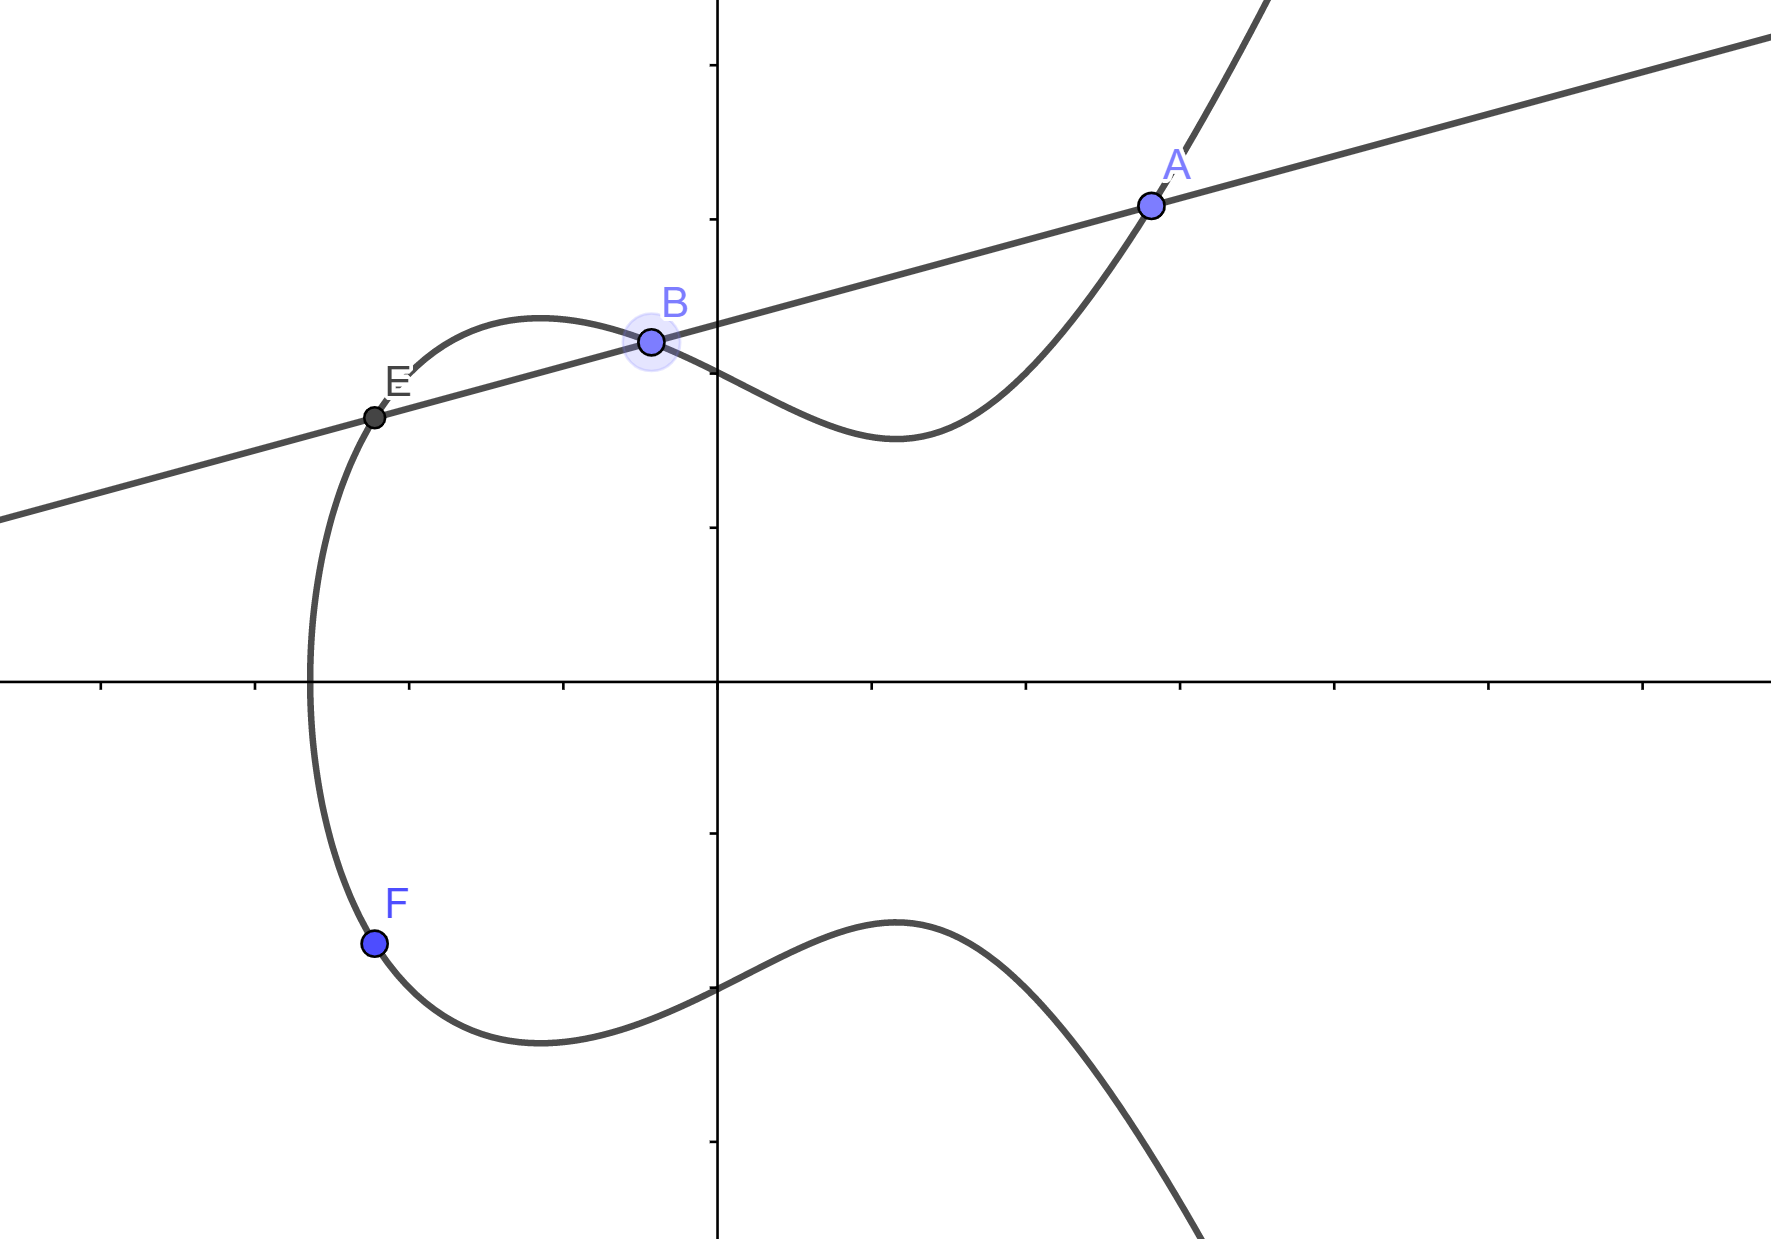
\includegraphics[width=15cm]{graphics/ec_summation.png}
\end{figure}
\begin{figure}[!ht]
\caption{Иллюстрация операции удвоения на эллиптических кривых.}\label{fig:ec_doub}
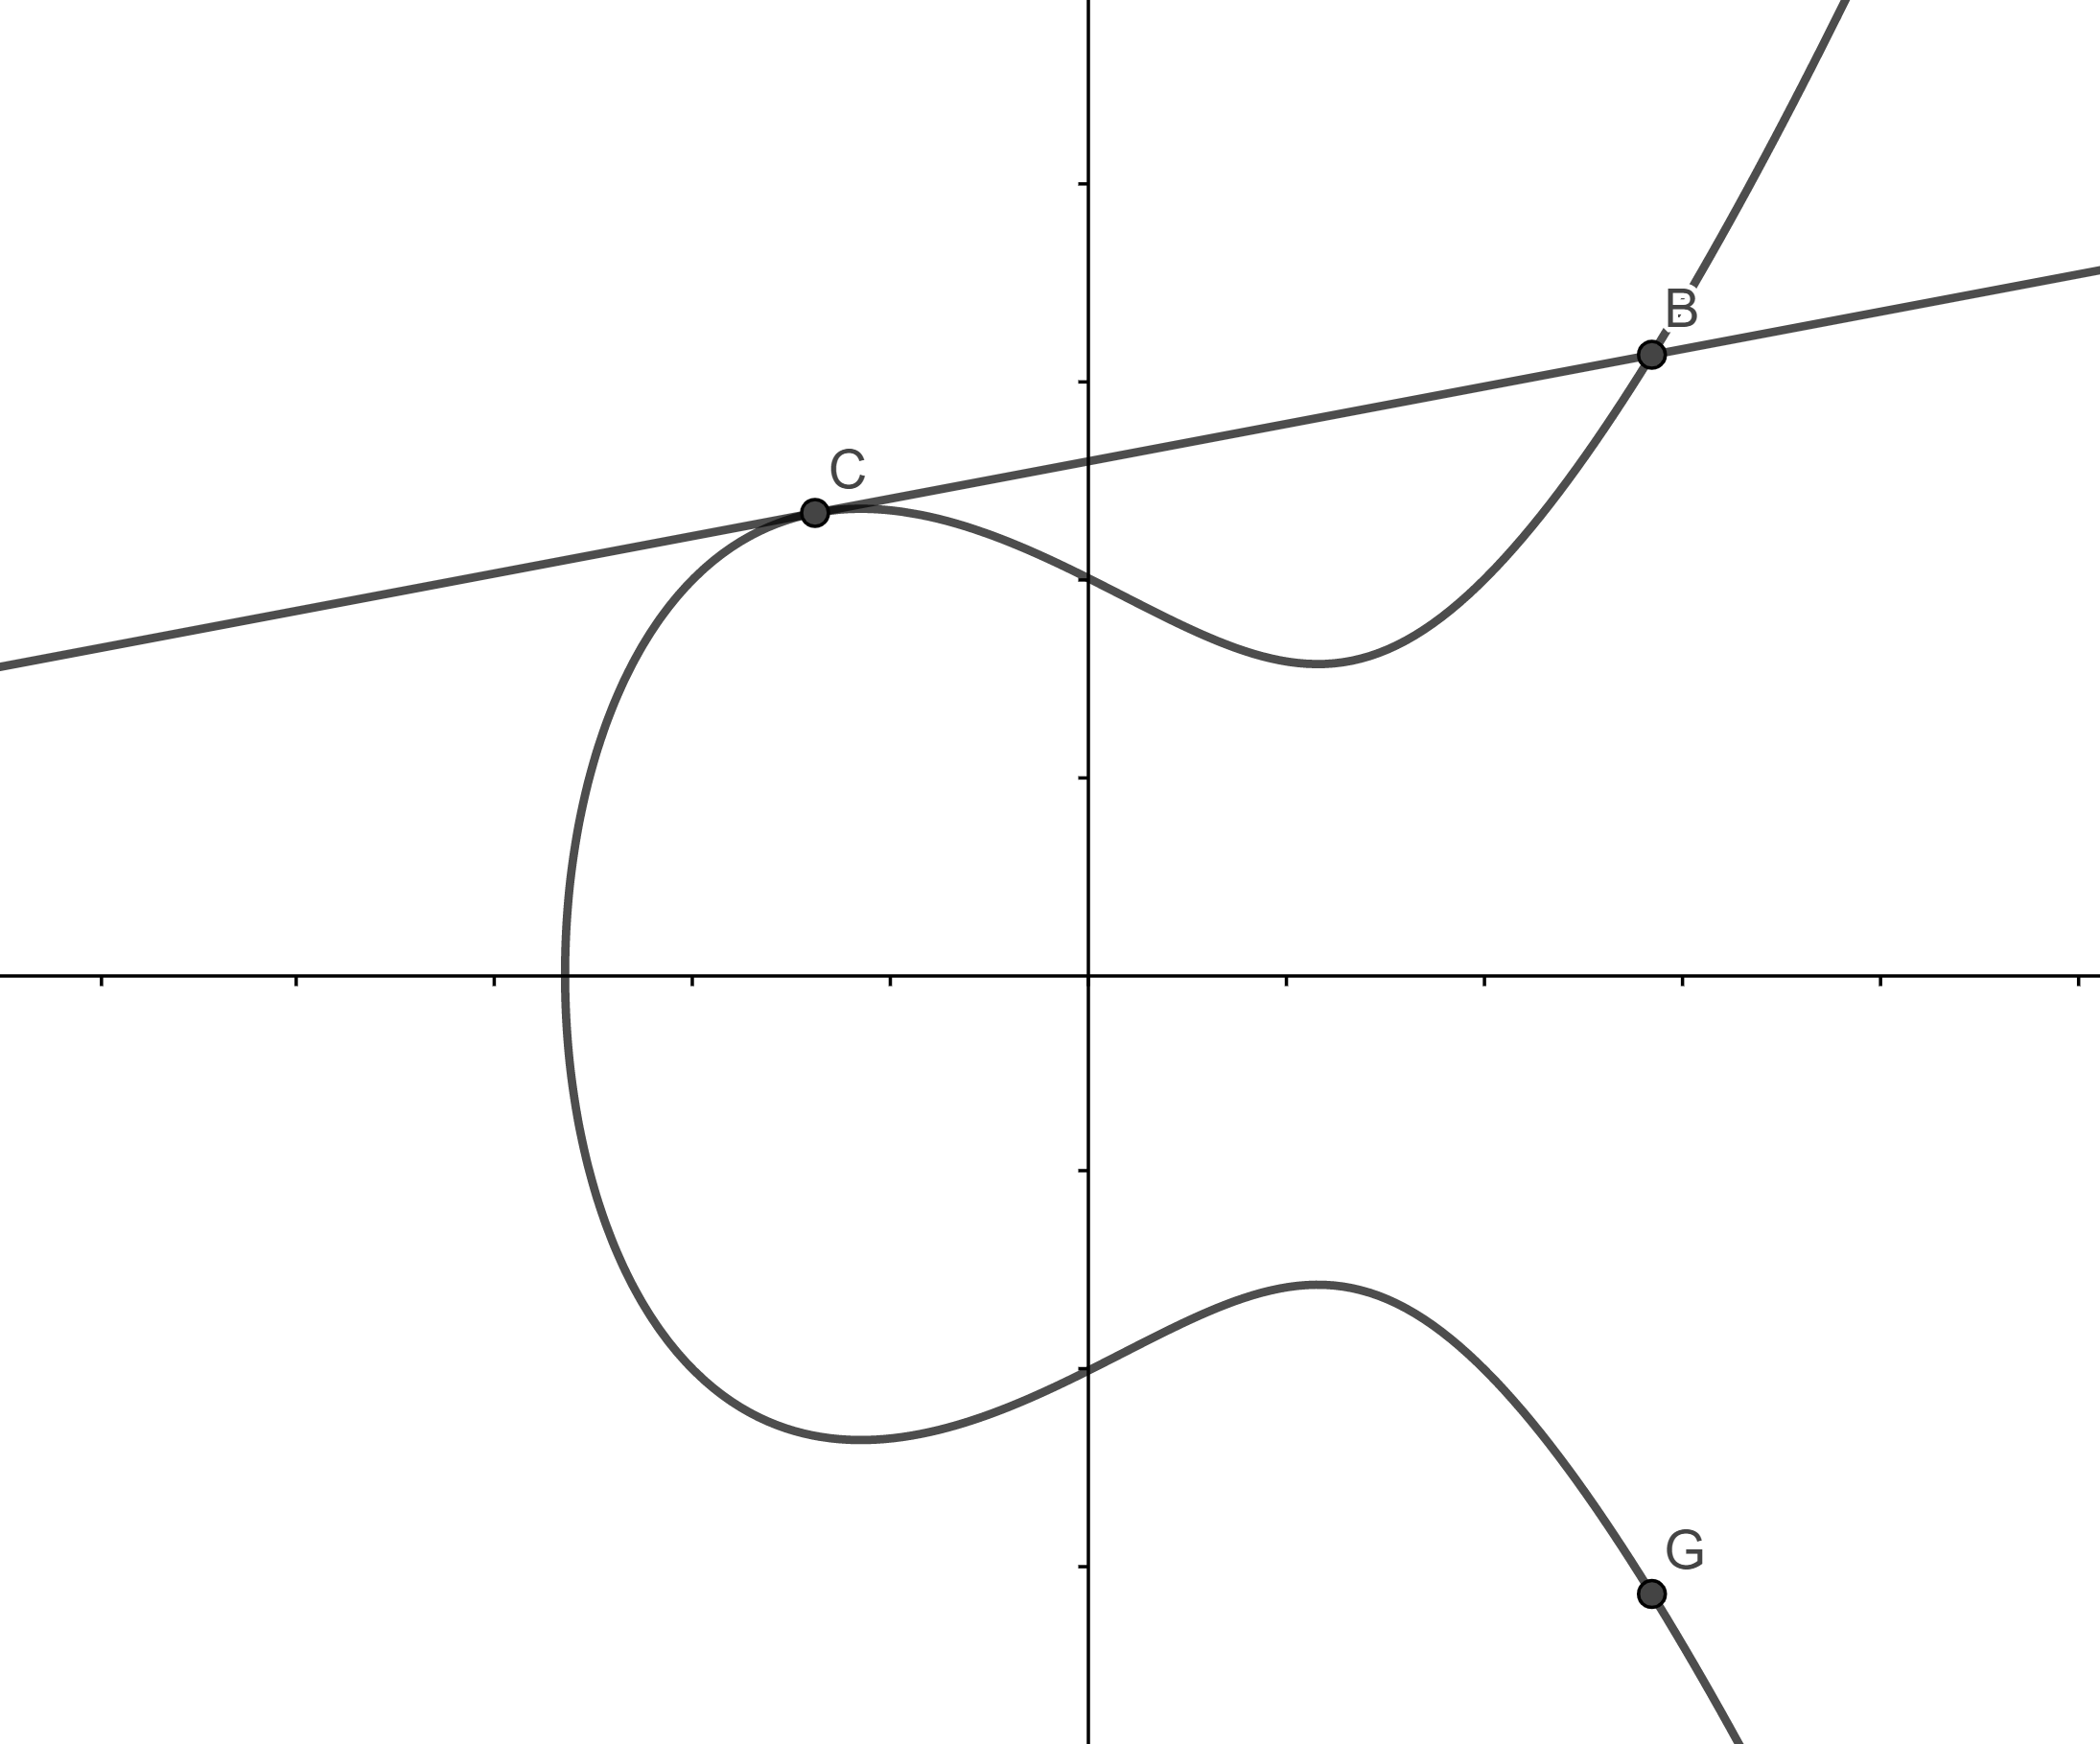
\includegraphics[width=15cm]{graphics/ec_doubling.png}
\end{figure}
Также в современной криптографии как односторонняя функция широко используется умножение на эллиптических кривых.
Эллиптическая кривая - это набор точек в конечном поле, подходящих под уравнение $y^2=x^3+ax+b$.
Умножение определено как повторяющееся $n$ раз сложение точки $P=(x,y)$, лежащей на этой кривой: $nP=P+P+\dots+P$
Сложение на эллиптической кривой можно описать как проведение линии через две точки, а затем отражение точки пересечения этой линии с кривой.
Если посмотреть на рисунок~\ref{fig:ec_sum}, то $A+B=-E=F$.
Для ускорения умножения можно использовать операцию удвоения, которую можно описать как проведение касательной к точке и
отражение точки пересечения касательной и кривой.
Если посмотреть на рисунок~\ref{fig:ec_doub}, то $C+C=-B=G$.
За счёт удвоения можно сократить количество операций с $n$ умножений до $log_2 n$ удвоений и небольшого числа умножений.
Это аналогично методу оптимизации <<возводи в квадрат и умножай>> для возведения числа в степень, который будет раскрыт в главе~\ref{sec:exp}.
На эллиптических кривых задача,обратная к умножению, также называется задачей дискретного логарифмирования.
Но на эллиптических кривых она решается за экспоненциальное время, то есть она сложнее, чем аналогичная задача на конечных полях.
За счёт этого в криптографии на эллиптических кривых используются ключи гораздо меньшего размера для той же сложности.\par
Несмотря на это, из-за сложностей реализации криптографии на эллиптических кривых чаще используется криптография на конечных полях.
Поэтому в данной работе рассматривается оптимизация именно для конечных полей $GF(2^k)$, которые подробно рассмотрены в главе~\ref{sec:fields}.


\section{Алгоритм Диффи-Хеллмана}\label{sec:dhke}

Здесь будет подробное объяснение алгоритма~\cite{dif77}, раскрывающее аналогию из введения.
Также будет повторный акцент на широком использовании алгоритма и его недостатках~\cite{adr15},
которые делают необходимым использование более надёжных ключей и оптимизации.

 Уитфилдом Диффи и Мартином Хеллманом, а также независимо от них Ральфом Мерклом


\section{Клеточные автоматы}\label{sec:cells}

В этой главе будет рассказано о клеточных автоматах, их истории и структуре.
Также будет рассказано об их применениях в криптографии.
Как источники будут использоваться~\cite{zhu17, zhu17_2}.

\section{Конечные поля}\label{sec:fields}

Здесь будут описаны конечные поля в общем и их применение в криптографии.
Также будет рассказано конкретно о полях GF($2^k$) и их особенностях при имплементации на ЭВМ.
Будут приведены примеры других имплементаций.
Как источники будут использоваться~\cite{pri16, mau15, knu97_2}.

\section{Умножение в конечных полях}\label{sec:mult}

Тут вкратце будет рассказано об алгоритмах умножения в конечных полях.
Также будет объяснён крестьянский алгоритм, который используется для умножения в моей имплементации.
Источниками будут~\cite{knu97, men01, koc98}.

\section{Алгоритмы возведения в степень по модулю}\label{sec:exp}

Здесь будут представоены алгоритмы left-to-right и описание различных имплементаций и проблем.
Источниками будут~\cite{knu97, men01, koc97}.
\section{Алгоритм Монтгомери}\label{sec:mont}

Здесь будет описание алгоритма и формы Монтгомери, а также принципы, благодаря которым этот способ быстрее.
Также будет представлено описание адаптации алгоритма на клеточные автоматы, с помощью которой
возможна реализация на
Источниками будут~\cite{jeo07, men01, koc97}.

\section{Параллелизация алгоритма Монтгомери}\label{sec:paramont}

Здесь будет пересказ статьи~\cite{ku04} с подробным описанием алгоритма.
Также будет объяснение перевода алгоритма на клеточные автоматы.
Клеточные автоматы в рамках данной работы - это абстракция, позволяющия объяснить алгоритм.
Но эта абстракция ценна тем, что с её использованием можно создать реализацию "в железе" с логическими элементами.

\finishrelatedwork
\chapterconclusion

Будут подведены итоги, объяснён выбор конкретных алгоритмов (основной использующийся, стандартный
Монтгомери и параллелизация Монтгомери) и приведены теоретические прогнозы по приросту производительности
из источников.

\chapter{Имплементация и тестирование}

\section{Выбор языка программирования}\label{sec:prog}

Будет рассказано про особенности языка Python, за которые он был выбран для данного проекта.
В частности, про то, что в Python переменные и числа не имеют ограничения по длинне, что делает
возможным тестирование на очень длинных ключах.
Также будут описаны альтернативы (performance-focused implementations из статьи) и их недостатки.

\section{Описание имплементации}\label{sec:impl}

Здесь будет не очень много, в основном структура и ссылки на алгоритмы из первой главы.
В приложении будет код - не весь, но некоторых функций.
Возможно, будут ссылки на упомянутые ранее альтернативы.

\section{Методология тестирования производительности}\label{sec:meth}

Ссылки на наборы многочленов~\cite{rfc7296, rfc3526} и повторный рассказ о методиках их выбора~\cite{rfc2412}.
Также упор на многократное тестирование на случайных числах.
Тут в основном, опять же, из статьи.

\section{Результаты тестирования производительности}\label{sec:results}

Графики из статьи на русском и их описание.

\chapterconclusion

Подробный разбор результатов тестирования с акцентом на приросте в производительности почти в полтора раза.

\startconclusionpage

Краткое описание достигнутых результатов, акцент на возможности реализации "в железе"
и минимальности изменений для программной.
Также акцент на том, что прирост в производительности универсален и может быть применён не только для Диффи-Хеллмана
как further research.

\printmainbibliography


\appendix

\chapter{Секции исходного кода имплементации}\label{sec:app:1}

    Некоторые критические функции и ссылка на репозиторий.

\end{document}
